\chapter{Volume rendering on mobile devices (Virtual Reality, Augmented Reality, Mixed Reality) }
\label{mixedReality}

This chapter presents the research I have started at the end of this thesis. 
We address the volume rendering challenges on mobile devices (Virtual reality, augmented reality, and mixed reality). Mobile devices are getting more and more popular across the population. Although their technical specifications can be totally different from one device to another, they are all becoming more powerful int terms of memory, CPU, GPU, and features.

\section{Introduction}

First of all, let us define and be more following terms: virtual reality, augmented reality, and mixed reality.

\par \textbf{ Virtual Reality (VR)} immerses users in a fully artificial digital environment. In fact, This technology immerses users in a completely virtual environment that is generated by a computer. The most advanced VR experiences even provide freedom of movement – users can move in a digital environment and hear sounds. Moreover, special hand controllers can be used to enhance  virtual reality experiences.\newline
You need to wear a special VR headset to experience virtual reality. Most VR headsets are connected to a computer (Oculus Rift) or a gaming console (PlayStation VR) but there are standalone devices (Google Cardboard is among the most popular) as well. Most standalone VR headsets work in combination with smartphones: the user insert a smartphone into a headset, then wear this headset, and immerse in the virtual reality.

\par \textbf{Augmented Reality (AR)} allows users to see and interact with the real world while digital content is added to it. As a popular example, we can think of Pokemon Go which causes millions of people all over the world have been rushing with their smartphones in search for small virtual creatures. That is the most pertinent example of augmented reality. \newline
If you own a modern smartphone, you can easily download an AR app and try this technology. There is a different way to experience augmented reality, though  with special AR headsets, such as Google Glass, where digital content is displayed on a tiny screen in front of a user's eye.

\par \textbf{Mixed Reality (MR)} is the most recent development in reality technologies that sometimes causes confusion, primarily because different experiences are called so. Without going too deep into science, let us look at two forms of reality technologies that are referred to as mixed reality (As I have mentioned just one of them at the very beginning):

\begin{itemize}

\item \textbf{ Mixed reality that starts with the real world }– virtual objects are not just overlaid on the real world but can interact with it. In this case, a user remains in the real-world environment while digital content is added to it; moreover, a user can interact with virtual objects. This form of mixed reality can be considered an advanced form of AR.

\item  \textbf{Mixed reality that starts with the virtual world} – the digital environment is anchored to and replaces the real world. In this case, a user is fully immersed in the virtual environment while the real world is blocked out. It almost looks like virtual reality. In fact it does, but the digital objects overlap the real ones whereas in conventional VR the virtual environment is not connected to the real world around a user. To experience this form of mixed reality, you can wear Windows mixed reality headsets. 
\end{itemize}

\section{Stereoscopic 3D}

Stereoscopic 3D is used in virtual reality and  mixed reality systems.
This  is a technique that produces an illusion of depth in a moving image by displaying two slightly different images to the right and left eye of the observer . This ability is based on the characteristics of the human visual system. The eyes, being positioned horizontally in the head, receive two views of the visual scene - one for the left-eye and another for the right-eye. The views overlap but differ slightly since they originate from two distinct perspectives. The visual system interprets and processes the information gathered from the two images to produce stereoscopic depth. The binocular system is very good at coordinating the movement of the eyes, which move constantly even during fixation. From a functional point of view, the images of both eyes fall on the fovea when fixating binocularly on a point. 


The fovea is the part of the back of the eye that has the highest acuity. According to \cite{5743036}, ''an object fixated binocularly is imaged on the same relative coordinates in the left-eye and right-eye views and it is perceived as a single percept, i.e., it is seen as a single object.''



To look at a new object located at a different distance, the point of fixation is altered. The two eyes move at the same time and in opposite directions so that the new object is imaged in the center of each eye's fovea. When the new object is closer the eyes move inward (convergence). On the contrary, when the new object is farther away the eyes move outward (divergence). This process is called vergence and it is related to accommodation

\section{ Virtual Reality (VR)}

There are two main types of VR headsets: PC-connected headsets and Standalone headsets. Each type influences differently the volume rendering process according to its specifications.


\subsection{PC-connected headsets}

As their name suggests, these VR headsets are connected to a computer (or a gaming console) that generates high-quality virtual experiences. The processing power of modern computers is huge, so they can generate realistic and persuasive digital worlds. This characteristics are really interesting for volume rendering since direct volume rendering is greedy in term of processing. The more processing capability available, the more quality we will get at the end of the rendering pipeline. 

Another major constraint with virtual reality in general is the necessity to render two different image to create an illusion of depth thanks to stereoscopic 3D.


VR headsets can be used along with special controllers. In this case, users can actually interact with the virtual environment they are immersed in. As might be expected, PC-connected headsets provide the most engaging VR experiences.

The most popular PC-connected VR headsets are HTC Vive, PlayStation VR, and Oculus Rift.

HEEEEEEEEEEEEERRRRRRRRRRRRRRRRRRRRE

\subsection{Standalone headsets}

Until now, PC-connected VR headsets are quite expensive and relatively few people are willing to invest their money in them. Yet there is another way to experience virtual reality – using standalone headsets that do not need to be connected to a computer or console.

Most standalone VR headsets use a smartphone screen to provide the virtual reality experience. Such devices are quite affordable, as users can simply insert their smartphone into the headset to enjoy VR. Samsung Gear VR, Google Daydream, and Google Cardboard work exactly this way.

Other standalone headsets work on their own. Facebook's soon-to-be-released Oculus Go, for example, will need neither a computer nor a smartphone to generate virtual experiences. This device is likely to make virtual reality technology a lot more common and affordable than it is now.

This standalone headsets are then more susceptible to have a larger user population than the PC-connected ones. It is then really appropriate to investigate how the volume rendering process can be well implemented and adapted to this kind of devices. However, due to the less powerful graphical process unit available in theses standalone devices, we have to find a better trade-off between the frame rate and the quality of the rendered image. 


\section{ Augmented Reality (AR)}

Augmented reality (AR) is the overlay of digital content on the real-world environment. Virtual objects can be in various forms: images, videos, or interactive data.


In other words, if you see the real world supplemented with digital objects, that is AR. Imagine you want to buy a piece of furniture – a chair, for example. Augmented reality technology can help you check how different chairs will look in your room and pick the one that fits best.


So how can you bring AR experiences to life? There are two main ways: Portable devices and Smart glasses and AR headsets. 


\subsection{Portable devices}

Augmented reality is the most accessible reality technology, as people can use their smartphones or tablets to run augmented reality applications. AR apps use a phone camera to capture the real world; virtual objects are then overlaid and users can see them on their smartphone screen.


That is how common AR apps work, the best example being Pokemon Go. Millions of people have used their smartphones to play this game and catch virtual Pokemons that they can only see on their smartphone screens. 


Since smartphones are extremely affordable now, augmented reality could bring more experience into the visualization of volumetric datasets. 

HEEEEEEEEEEEEERRRRRRRRRRRRRRRRRRRRE

\subsection{Smart glasses and AR headsets}

Another way to create AR experiences is to use special smart glasses or headsets. Unlike VR headsets, these AR glasses and headsets do not immerse users into a fully virtual environment but just add digital objects to the real world. With Google Glass, for example, digital data is projected right in front of the user's eyes.

\section{ Mixed Reality (MR)}

In mixed reality (sometimes called hybrid reality), virtual content is not only overlaid on the real environment (as in AR) but is anchored to and interacts with that environment.

In a nutshell, with mixed reality you can see virtual objects just like you can with augmented reality, but these objects can also interact with the real world. In a sense, mixed reality is a more immersive and interactive type of augmented reality.

There can be, however, a different form of mixed reality – when users see and interact with a completely virtual environment overlaid on the real world around them.

However, a common issue is to trip over a physical object in the room while interacting with a completely digital environment.
To avoid this problem, a headset must be able to track the real world and adjust the virtual environment accordingly. This kind of mixed reality is closer to VR than AR; in fact, some VR headsets have sensors to track the physical environment too. Different types of devices are required to experience these two forms of mixed reality:

\begin{itemize}
 \item \textbf{ Holographic devices: } These headsets have translucent glasses that allow you to perfectly see your surroundings. Virtual experiences are created with the help of holograms. That is how Microsoft HoloLens works.
 
 \item \textbf{ Immersive devices:} These headsets have non-translucent displays that completely block out the real world (just like VR headsets) and use cameras for tracking. Windows mixed reality headsets from Acer and HP work this way.

\end{itemize}

\subsection{Implementation}

During the end of this thesis, we begin to implement a volume rendering framework on a Holographic device. We use an Hololens (see \cite{hololens}) as the holographic design to support the volume renderer framework. We tried two different types of implementations. The first one and the least difficult is to compute and render the volume on the holographic device itself. The second type of implementation is to use the \textbf{ "remoting" } strategy. The remoting strategy allow to do all the computation on a computer (usually more powerful than the holographic device) and send the final images (one for each eye) through the WiFi to be rendered on the Hololens.

\subsubsection{Computation on the hololens}

The GPU of the hololens is not really powerful and as a low memory capacity (around 600 MB).  Knowing that the default and maximum supported resolution is 720p (1268x720) for each eye, have to compute two images with a lower resolution than this maximum value.  To develop an holographic app, one can either use the Unity framework or directly develop an universal holographic application using Visual studio and directX.


Using the Unity framework to develop an holographic application is quite simple. We test different types of volume rendering algorithms: rayasting, 3D textures, and isosurfaces.
We used Cg/HLSL in Unity to speed up the rendering process. Although the final result was beautiful, the prototype was not interactive because of low frame rates (between 1 and 5) according to the algorithm used and the different parameters such as the number of isosurfaces, the step during raycasting, or the number of slices computed when using 3D textures.


The second solution was to directly develop an universal holographic application using Visual studio and directX. It help us to gain more speed and frame rate than the unity version of each of these algorithms (see \autoref{fig:mixediso}, and \autoref{fig:mixedray}). 

\begin{figure}
\centering
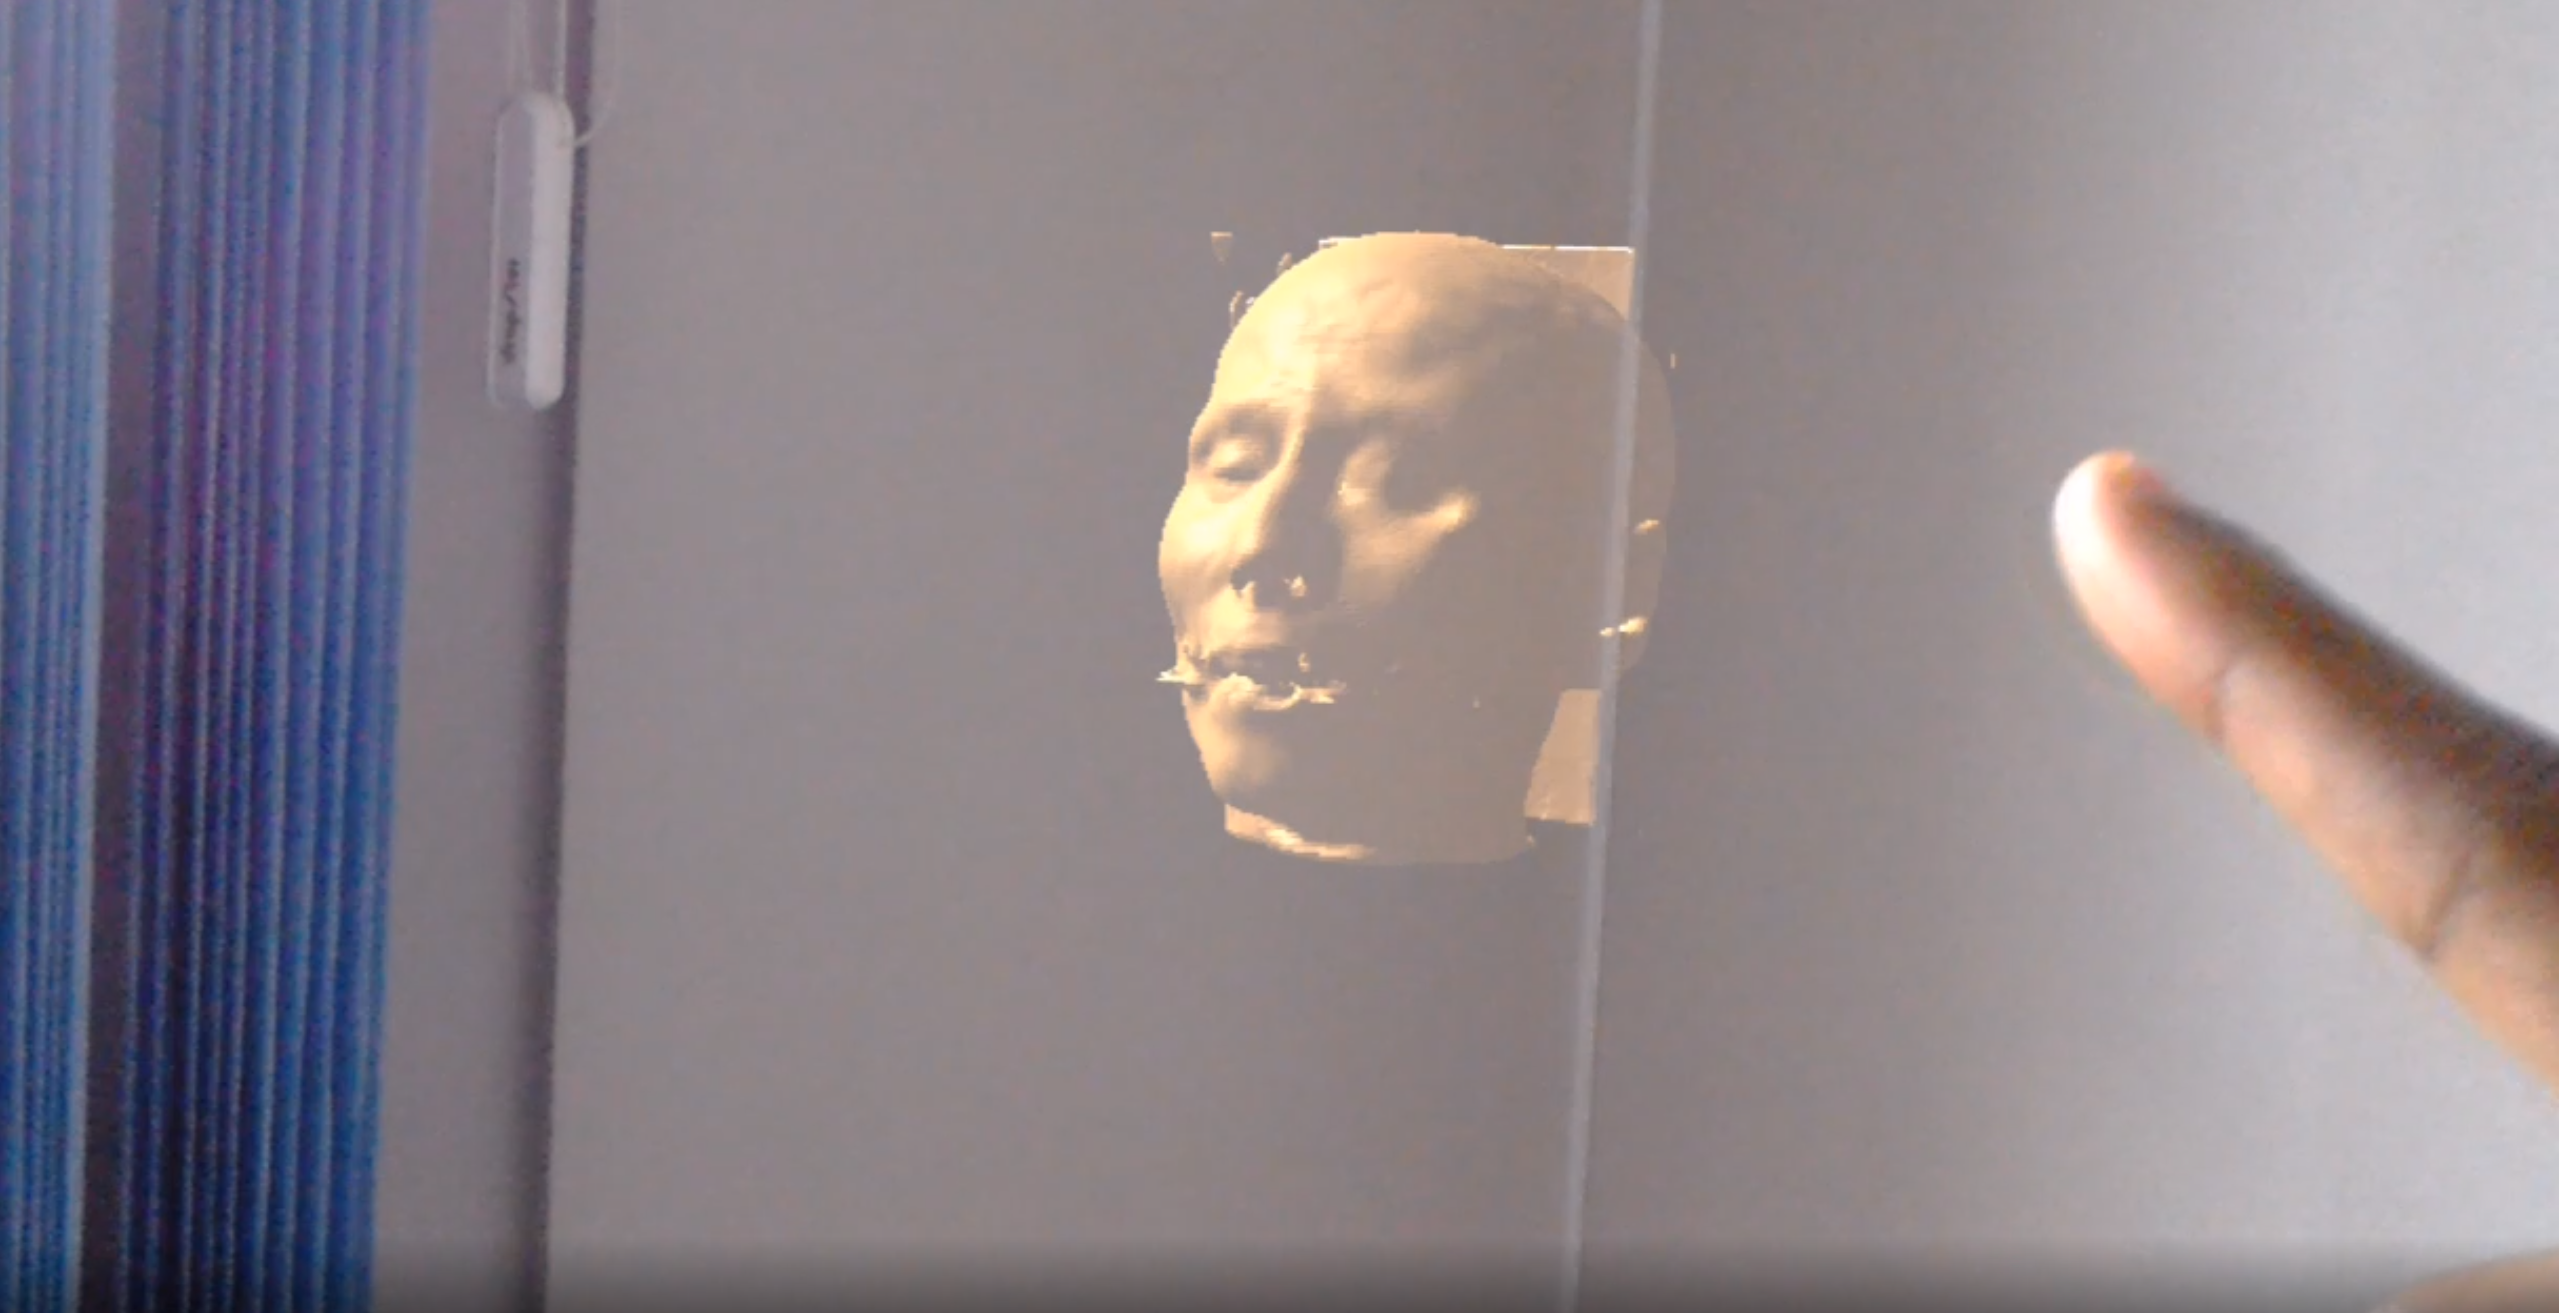
\includegraphics [width=\textwidth]{Figures/mixediso}
\caption{A head CT scan rendered on the hololens using isosurfaces }
\label{fig:mixediso}
\end{figure}


\begin{figure}
\centering
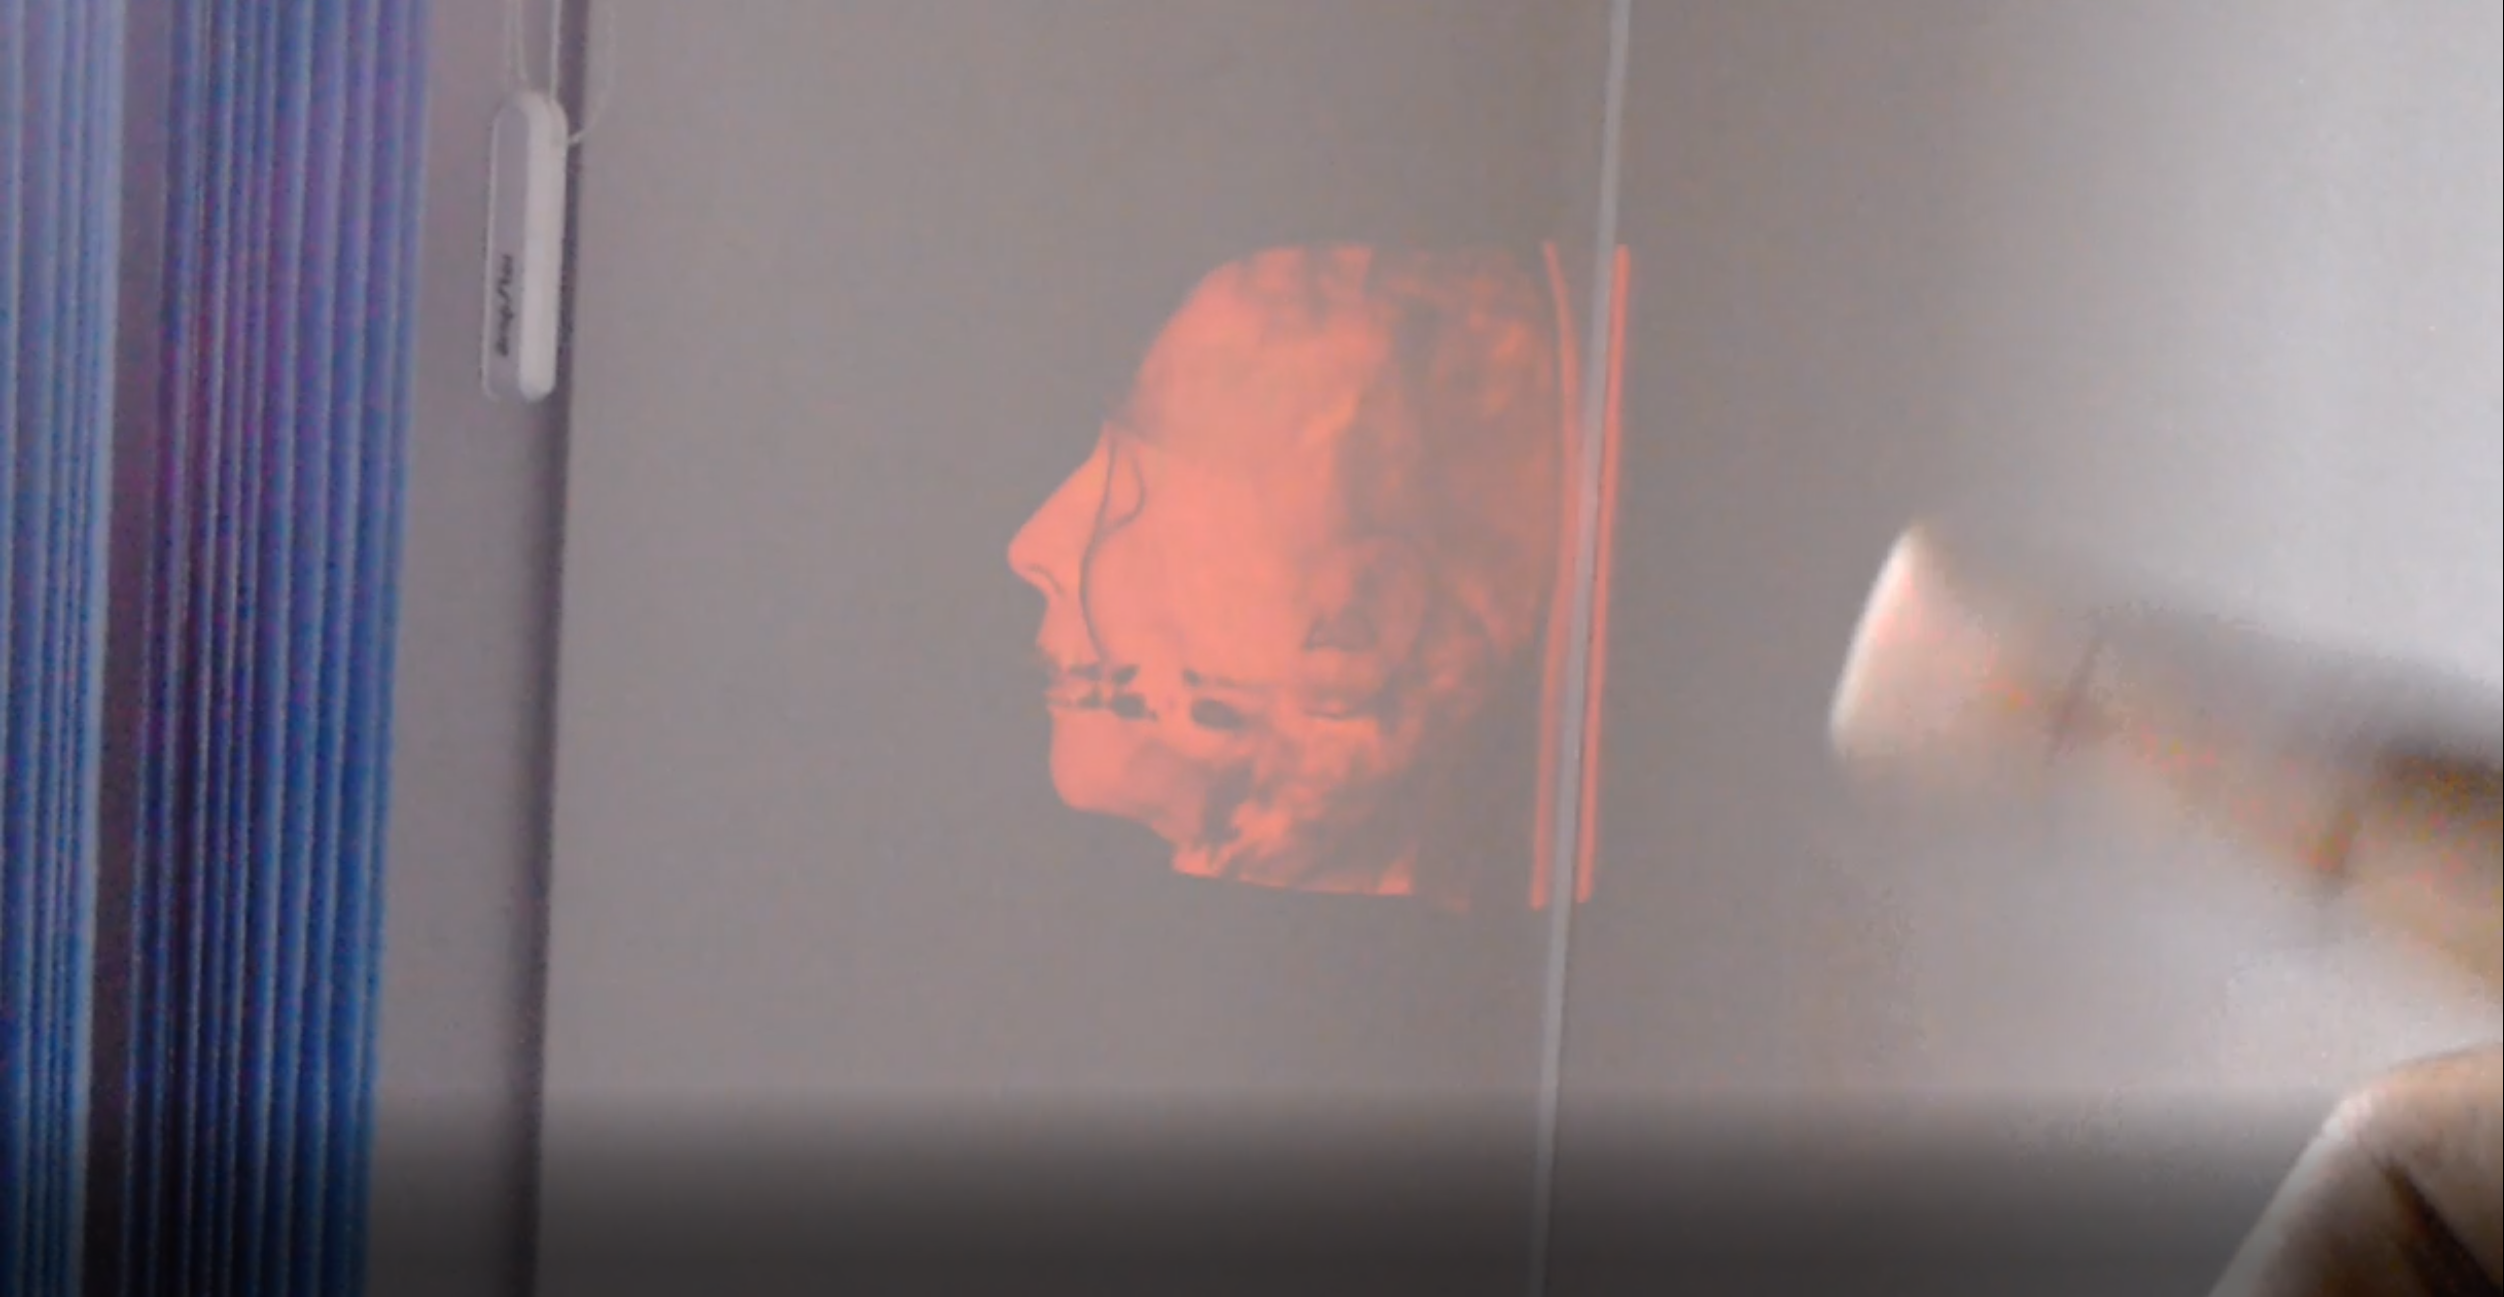
\includegraphics [width=\textwidth]{Figures/mixedray}
\caption{A head CT scan rendered on the hololens using a raycasting algorithm }
\label{fig:mixedray}
\end{figure}

We just develop some basic interactions so far. For instance we switch from the isosurface representation to the one using the raycasting algorithm by using the \textbf{"air tap"} gesture. Air tap is a tapping gesture with the hand held upright, similar to a mouse click or select. This is used in most HoloLens experiences for the equivalent of a "click" on a UI element after targeting it.  We use the \textbf{manipulation} gesture to modify the transfer function presets when using the raycasting algorithm.

\subsubsection{ Holographic remoting }